\chapter{The Derivative: Rates of Change of a Function}
\label{ch:derivatives}

\section{Slopes and Average Rates of Change}
\label{sec:slope}

Precalculus Idea: Slope and Rate of Change
The slope of a line measures how fast a line rises or falls as we move from left to right along the line. It measures the rate of change of the y-coordinate with respect to changes in the x-coordinate. If the line represents the distance traveled over time, for example, then its slope represents the velocity. In the figure, you can remind yourself of how we calculate slope using two points on the line:

slope
m=Slope from P to Q=riserun=y2-y1x2-x1=ΔyΔx
We would like to be able to get that same sort of information (how fast the curve rises or falls, velocity from distance) even if the graph is not a straight line. But what happens if we try to find the slope of a curve, as in the figure below?

slope
We need two points in order to determine the slope of a line. How can we find a slope of a curve, at just one point? The answer, as suggested in the figure, is to find the slope of the tangent line to the curve at that point. Most of us have an intuitive idea of what a tangent line is. Unfortunately, “tangent line” is hard to define precisely.

Definition (Secant Line)
A secant line is a line between two points on a curve

See the image below:

secant

\section{Tangent Lines and Instantaneous Rates of Change}
\label{sec:tangents}

%\section{Business Applications of Slope}
\label{sec:basic-apps}

Business and Economics Terms
Next we will delve more deeply into some business applications. To do that, we first need to review some terminology.

Suppose you are producing and selling some item. The profit you make is the amount of money you take in minus what you have to pay to produce the items. Both of these quantities depend on how many you make and sell. (So we have functions here.) Here is a list of definitions for some of the terminology, together with their meaning in algebraic terms and in graphical terms.

Cost
Your cost is the money you have to spend to produce your items.

Fixed Cost
The Fixed Cost (FC) is the amount of money you have to spend regardless of how many items you produce. FC can include things like rent, purchase costs of machinery, and salaries for office staff. You have to pay the fixed costs even if you don’t produce anything.

Total Variable Cost
The Total Variable Cost (TVC) for q items is the amount of money you spend to actually produce them. TVC includes things like the materials you use, the electricity to run the machinery, gasoline for your delivery vans, maybe the wages of your production workers. These costs will vary according to how many items you produce.

Total Cost
The Total Cost (TC, or sometimes just C) for q items is the total cost of producing them. It’s the sum of the fixed cost and the total variable cost for producing q items.

Average Cost
The Average Cost (AC) for q items is the total cost divided by q, or TCq. You can also talk about the average fixed cost, FCq, or the average variable cost, TVCq.

Marginal Cost
The Marginal Cost (MC) at q items is the cost of producing the next item. Really, it’s
MC(q)=TC(q+1)-TC(q).
In many cases, though, it’s easier to approximate this difference using calculus (see Example \ref{ex:2-7-11} below). And some sources define the marginal cost directly as the derivative,
MC(q)=TC′(q).
In this course, we will use both of these definitions as if they were interchangeable.

The units on marginal cost is cost per item.

Why is it okay that there are two definitions for Marginal Cost (and Marginal Revenue, and Marginal Profit)?

We have been using slopes of secant lines over tiny intervals to approximate derivatives. In this example, we’ll turn that around – we’ll use the derivative to approximate the slope of the secant line.

Notice that the “cost of the next item” definition is actually the slope of a secant line, over an interval of 1 unit:
MC(q)=C(q+1)-1=C(q+1)-11.
So this is approximately the same as the derivative of the cost function at q:
MC(q)=C′(q).
In practice, these two numbers are so close that there’s no practical reason to make a distinction. For our purposes, the marginal cost is the derivative is the cost of the next item.

\begin{example}
The table shows the total cost (TC) of producing q items.

Items, q	TC	0	\$20,000	100	\$35,000	200	\$45,000	300	\$53,000
What is the fixed cost?
When 200 items are made, what is the total variable cost? The average variable cost?
When 200 items are made, estimate the marginal cost.

\begin{solution}
  The fixed cost is \$20,000, the cost even when no items are made.
When 200 items are made, the total cost is \$45,000. Subtracting the fixed cost, the total variable cost is \$45,000 - \$20,000 = \$25,000.

The average variable cost is the total variable cost divided by the number of items, so we would divide the \$25,000 total variable cost by the 200 items made. \$25,000/200 = \$125. On average, each item had a variable cost of \$125.

We need to estimate the value of the derivative, or the slope of the tangent line at q=200. Finding the secant line from q=100 to q=200 gives a slope of
45,000-35,000200-100=100.
Finding the secant line from q=200 to q=300 gives a slope of
53,000-45,000300-200=80.
We could estimate the tangent slope by averaging these secant slopes, giving us an estimate of \$90/item.

This tells us that after 200 items have been made, it will cost about \$90 to make one more item.
\end{solution}\end{example}
 % Cut this section.
\section{The Derivative}
\label{sec:derivative}

\subsection{Derivative Concepts and Notation}

\begin{definition}
We can view the {\bf derivative}\index{Derivative} of a function, $f(x)$ in several different equivalent ways. Here are a three of them. The derivative of $f(x)$ at a point $(a, f(a))$ is:
    \begin{itemize}
    \item the instantaneous rate of change of $f(x)$ at $x=a$, 
    \item the slope of the tangent line to the graph of $f(x)$ at the point $(a,f(a))$, and
    \item the slope of the curve $y=f(x)$ at the point $(a,f(a))$.
    \end{itemize}
\end{definition}

We've been acting as if derivatives exist everywhere for every function. This is true for most of the functions that you will run into in this textbook. But there are some common places where the derivative doesn't exist.

\begin{definition}
A function, $f(x)$, is called {\bf differentiable}\index{Differentiable} at the point $(a,f(a))$ if its derivative exists at $x=a$.
\end{definition}

Remember that the derivative is the slope of the tangent line to the curve. That's what to think about.

Where can a slope not exist? If the tangent line is vertical, the derivative will not exist.

\begin{example}
Show that $f(x)=\sqrt[3]{x}=x^{1/3}$ is not differentiable at $x=0$.

\begin{solution} From the graph in Figure \ref{fig:2-3-cuberoot}, we can see that the tangent line to $y=\sqrt[3]{x}$ at $x=0$ is vertical with undefined slope, which is why the derivative does not exist at $x=0$.

\begin{figure}[!ht]
  \centering
    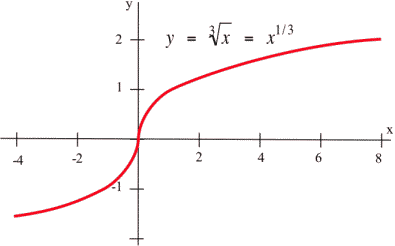
\includegraphics[width=0.4\textwidth]{img/chap2/image037.png}
    \caption{$f(x)=\sqrt[3]{x}$}
    \label{fig:2-3-cuberoot}
\end{figure}
\end{solution}\end{example}

Where can a tangent line not exist?

If there is a sharp corner (cusp)\index{Cusp} in the graph, the derivative will not exist at that point because there is no well-defined tangent line (a teetering tangent, if you will).

If there is a discontinuity\index{Discontinuity} in the graph (a jump, a break, a hole in the graph, or a vertical asymptote), the tangent line will be different on either side and the derivative will not exist at that point.

\begin{example}
Show that $f(x)=|x|$ is not differentiable at $x=0$.

\begin{solution} On the left side of the graph in Figure \ref{fig:2-3-absx}, the slope of the line is $-1$. On the right side of the graph, the slope is $1$. There is no well-defined tangent line at the sharp corner at $x=0$, so the function $|x|$ is not differentiable at that point.

\begin{figure}[!ht]
  \centering
    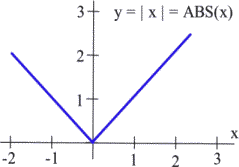
\includegraphics[width=0.4\textwidth]{img/chap2/image038.png}
    \caption{$f(x)=|x|$}
    \label{fig:2-3-absx}
\end{figure}
\end{solution}\end{example}


\begin{definition}
When we find the derivative of a function, or take the derivative of a function, we say that we {\bf differentiate}\index{Differentiate} the function.
\end{definition}

\paragraph*{Notation for the Derivative}
Calculus was invented by Leibniz\index{Leibniz, Gottfried} and Newton\index{Newton, Isaac}, but it was developed by many more throughout the subsequent centuries. Many developed their own notation for the derivative of a function. The notation developed by Leibniz and Joseph-Louis Lagrange\index{Lagrange, Joseph-Louis} are the most convenient and most used. 

The derivative of $y=f(x)$, with respect to $x$, is written in many different ways:
\begin{itemize}
    \item $f'(x)$: ``$f$ prime of $x$'',
    \item $y'$: ``$y$ prime,''
    \item $\dfrac{dy}{dx}$: ``$d$ $y$ $d$ $x$,''  
    \item $\dfrac{df}{dx}$: ``$d$ $f$ $d$ $x$,'' or
    \item $\dfrac{d}{dx}f(x)$: ``$d$ $d$ $x$ of $f$ of $x$.''
\end{itemize}
The notation that resembles a fraction is called {\bf Leibniz notation}\index{Leibniz notation}. It displays not only the name of the function ($f$ or $y$), but also the name of the variable (in this case, $x$). It looks like a fraction because the derivative is a slope. In fact, this is simply $\dfrac{\Delta y}{\Delta x}$ written in Roman letters instead of Greek letters. The nuance here is that $\Delta v$\index{Delta} represents a finite difference of some variable $v$, whereas $dv$ represents an {\bf infinitesimal}\index{Infinitesimal} difference of a variable $v$. An infinitesimal difference would be a difference that is infinitely small, but not 0. That may sound like an oxymoron, but until about 1850, calculus was developed using infinitesimal differences, also called {\bf differentials}\index{Differential}. 

The best way to understand differentials is with an analogy: $1:\infty::dx:1$. Suppose you had a bin with an infinite number of balls and you throw one ball in. You still throw in a ball, but the total quantity of balls in the bin is unchanged. In the same way, if you have a line that is one inch long and you add on a line of length $dx$ inches, then the line is still one inch long, despite ``lengthening'' the line by $dx$.
 
\paragraph*{Looking Ahead}
We will figure out ways to compute exact values of derivatives from many kinds of functions in Sections \ref{sec:algderiv}-\ref{sec:chain}. If the function is given to you as a table or graph, you will still need to approximate the derivative of the function this way.

This is the foundation for the rest of this chapter. It's remarkable that such a simple idea (the slope of a tangent line) and such a simple definition (for the derivative $f'(x)$) will lead to so many important ideas and applications.

\subsection{The Derivative as a Function}
We now know how to find (or at least approximate) the derivative of a function for any $x$-value. This means that we can think of the derivative as a function too. That is the origin of the term ``derivative.'' The derivative of a function is a function that is derived from that function. The input of the derivative is the same as the function, but the output is the value of the derivative at that $x$ value and the units reflect the rate of change concept.

\begin{example}
Below is the graph of a function $y=f(x)$. We can use the information in the graph to fill in a table showing values of $f'(x)$:
\begin{figure}[!ht]
  \centering
    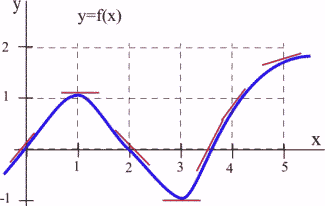
\includegraphics[width=0.4\textwidth]{img/chap2/image023.png}
    \caption{$y=f(x)$}
    \label{fig:2-3-fx}
\end{figure}

\begin{solution} At various values of $x$, draw your best guess at the tangent line and measure its slope. You might have to extend your lines so you can read some points. In general, your estimate of the slope will be better if you choose points that are easy to read and far away from each other. Here are estimates for a few values of $x$ (parts of the tangent lines used are shown above in the graph):
\begin{table}[ht!]
\begin{centering}
\begin{tabular}{ccc}
\toprule
$x$ &   $y=f(x)$    &	$f'(x)$\\
\midrule
0   &	0 &	1	\\
1   &	1 &	0	\\
2   &	0 &	$-1$  \\
3   &  $-1$ &	0	\\
3.5 &	0 &	2   \\
\bottomrule
\end{tabular}
\caption{Table of inputs, outputs, and derivatives of $f(x)$.}
\label{tab:2-3-deriv}
\end{centering}
\end{table}
Based on this, we can estimate the values of $f'(x)$ at some non-integer values of $x$ too: $f'(0.5)\approx   0.5$ and $f'(1.3)\approx   -0.3$.
\begin{figure}[!ht]
  \centering
    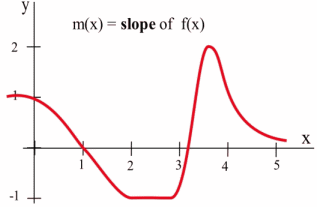
\includegraphics[width=0.4\textwidth]{img/chap2/image024.png}
    \caption{Slope of $y=f(x)$}
    \label{fig:2-3-fprimex}
\end{figure}
We can even think about entire intervals. For example, if $0<x<1$, then $f(x)$ is increasing; all the slopes are positive, and so $f'(x)>0$.

The values of $f'(x)$ definitely depend on the values of $x$, and $f'(x)$ is a function of $x$. We can use the results in the table to help sketch the graph of $f'(x)$.

\end{solution}\end{example}
\begin{example}
Figure \ref{fig:2-3-ht} shows the graph of the height, $h(t)$, of a rocket $t$ seconds after liftoff.

\begin{figure}[!ht]
  \centering
    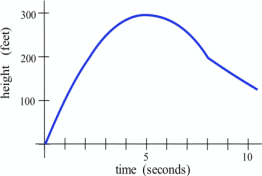
\includegraphics[width=0.4\textwidth]{img/chap2/image025.png}
    \caption{$y=h(t)$}
    \label{fig:2-3-ht}
\end{figure}
Sketch the graph of the velocity of the rocket at time $t$. (Velocity is the derivative of the height function, so it is the slope of the tangent to the graph of position or height.)

\begin{solution} We can estimate the slope of the function at several points. The graph in Figure \ref{fig:2-3-hprime} shows the velocity of the rocket. This is $v(t)=h'(t)$.

\begin{figure}[!ht]
  \centering
    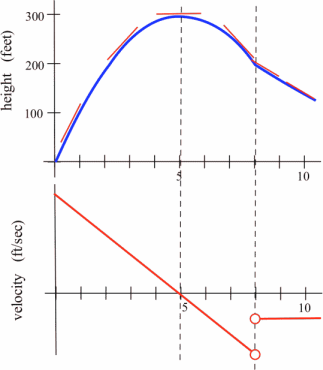
\includegraphics[width=0.4\textwidth]{img/chap2/image026.png}
    \caption{$y=h(x)$ and $y=h'(x)$}
    \label{fig:2-3-hprime}
\end{figure}
\end{solution}
\end{example}

\subsection{Interpreting the Derivative}
So far we have emphasized the derivative as the slope of the line tangent to a graph. That interpretation is very visual and useful when examining the graph of a function, and we will continue to use it. Derivatives, however, are used in a wide variety of fields and applications, and some of these fields use other interpretations. The following are a few interpretations of the derivative that are commonly used.

\paragraph*{General}

{\bf Rate of Change:} $f'(x)$ is the rate of change of the function at $x$. If the units for $x$ are years and the units for $f(x)$ are people, then the units for $\frac{df}{dx}$ are people per year, a rate of change in population.

\paragraph*{Graphical}

{\bf Slope:} $f'(x)$ is the slope of the line tangent to the graph of $f(x)$ at the point $(x,f(x))$.

\paragraph*{Physical}

{\bf Velocity:} If $f(x)$ is the position of an object at time $x$, then $f'(x)$ is the {\bf velocity}\index{Velocity} of the object at time $x$. If the units for $x$ are hours and $f(x)$ is distance measured in miles, then the units for $f'(x)=\frac{df}{dx}$ are miles per hour, which is a measure of velocity.

{\bf Acceleration:} If $f(x)$ is the velocity of an object at time $x$, then $f'(x)$ is the {\bf acceleration}\index{Acceleraton} of the object at time $x$. If the units are for $x$ are hours and $f(x)$ has the units miles per hour, then the units for the acceleration $f'(x)=\frac{df}{dx}$ are miles per hour per hour, or miles per hour$^2$.

\paragraph*{Business}

{\bf Marginal Cost}\index{Marginal cost}\index{Cost!marginal}, {\bf Marginal Revenue}\index{Marginal revenue}\index{Revenue!marginal}, and {\bf Marginal Profit}\index{Marginal profit}\index{Profitmarginal}: We introduced marginal cost in Section \ref{ssec:marginalcost} and marginal revenue and profit are defined in a similar way. In business contexts, the word ``marginal'' usually means the derivative or rate of change of some function. 

Therefore, {\bf marginal revenue}, $MR(n)$ is the additional revenue from selling one more item once we have already sold $n$ item. Just as with marginal cost, we will use both this definition and the derivative definition.
$$MR(n) = R(n+1)-R(n) \approx R'(n) \enspace.$$

{\bf Marginal profit} is the additional profit from selling one more item once we have already sold $n$ items. 
$$MP(n) = P(n+1)-P(n) \approx P'(n) \enspace.$$

If $f(x)$ is the cost to produce $x$ bicycles and the units for $f(x)$ are dollars, then the units for $f'(x)=\frac{df}{dx}$ are dollars per bicycle, the cost per bicycle.

One of the strengths of calculus is that it provides a unity and economy of ideas among diverse applications. The vocabulary and problems may be different, but the ideas and even the notations of calculus are still useful.

\subsection{Graphical Interpretations of the Basic Business Math Terms}
%Illustration
Figure \ref{fig:2-3-trandtc} shows graphs of $TR = R(q)$ and $TC = C(q)$ for producing and selling a certain item. The horizontal axis is the number of items, in thousands. The vertical axis is the number of dollars, also in thousands.

\begin{figure}[!ht]
  \centering
    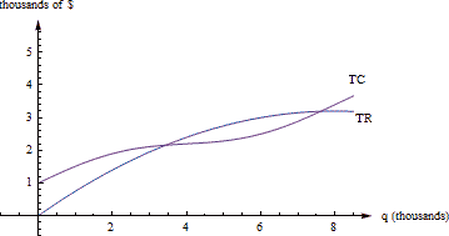
\includegraphics[width=0.4\textwidth]{img/chap2/image035.png}
    \caption{Total Revenue ($TR$) and Total Cost ($TC$) versus $q$ items.}
    \label{fig:2-3-trandtc}
\end{figure}
First, notice how to find the fixed cost and variable cost from the graph here. The fixed cost, $FC$, is the $y$-intercept of the $TC$ graph. ($FC=C(0)$.) The graph of variable costs would have the same shape as the graph of $TC$, shifted down.

Marginal cost for $q$ items is $MC(q)=C(q+1)-C(q)$, but that's impossible to read on this graph. How could you distinguish between $C(4022)$ and $C(4023)$? On this graph, that interval is too small to see, and our best guess at the secant line is actually the tangent line to the $TC$ curve at that point. (This is the reason we want to have the derivative definition handy.)
\begin{itemize}[label={}]
    \item $MC(q)$ is the slope of the tangent line to the $TC$ curve at the point $(q, C(q))$.
    \item $MR(q)$ is the slope of the tangent line to the $TR$ curve at the point $(q, R(q))$.
\end{itemize}
Profit is the distance between the $TR$ and $TC$ curves. If you experiment with a clear ruler, you'll see that the biggest profit occurs exactly when the tangent lines to the $TR$ and $TC$ curves are parallel. This is the rule that profit is maximized when $MR=MC$ which we'll explore in Section \ref{sec:app-opt}.

\begin{example}
Suppose the demand for widgets is $D(p)=\frac{1}{p}$, where $D$ is the quantity of widgets, in thousands, at a price of $p$ dollars. Approximate and interpret the derivative of $D$ at $p=\$3$.

\begin{solution} We can approximate $D'(3)$ by looking at a table, Table \ref{tab:2-3-Dprime}, of secant line slopes through the points $(3, D(3)) = \left(3, \frac{1}{3}\right)$ and $(3+\Delta p, D(3+\Delta p))$, where $\Delta p$ gets closer to $0$.

\begin{table}[ht!]
\begin{centering}
\begin{tabular}{lll}
\toprule
$\Delta p$ & $D(3+\Delta p)$ & $\dfrac{D(3+\Delta p)-D(3)}{\Delta p}$ \\
\midrule
1        & $\dfrac{1\mathstrut}{3+1\mathstrut} = 0.25$                & $\dfrac{D(4)     -D(3)}{1}     \approx -0.083333$ \\
0.1      & $\dfrac{1\mathstrut}{3+0.1\mathstrut} \approx 0.322581$    & $\dfrac{D(3.1)   -D(3)}{0.1}   \approx -0.107527$ \\
0.01     & $\dfrac{1\mathstrut}{3+0.01\mathstrut} \approx 0.332226$   & $\dfrac{D(3.01)  -D(3)}{0.01}  \approx -0.110742$ \\
0.001    & $\dfrac{1\mathstrut}{3+0.001\mathstrut} \approx 0.333222$  & $\dfrac{D(3.001) -D(3)}{0.001} \approx -0.111074$ \\
0.0001   & $\dfrac{1\mathstrut}{3+0.0001\mathstrut} \approx 0.333322$ & $\dfrac{D(3.0001)-D(3)}{0.0001}\approx -0.111107$ \\
\bottomrule
\end{tabular}
\caption{Average rate of change of demand approaching $D'(3)$.}
\label{tab:2-3-Dprime}
\end{centering}
\end{table}
Based on this, the quantities in the last column appear to be approaching $-0.1111\ldots$, which is $\frac{-1}{9}$. Later, we will show that that is indeed true. Since $D(p)$ has units ``thousands of widgets'' and the units for $p$ is ``dollars,'' the units for $D'(3)$ will be thousands of widgets per dollar. Therefore, $D'(3) \approx -0.111$ thousand widgets per dollar, or $-111$ widgets per dollar. This shows how the demand for widgets will change as the price increases.

Specifically, $D'(3)\approx -111$ widgets per dollar tells us that when the price of a widget is $\$3$, then the demand for widgets will decrease by about 111 widgets for every dollar the price increases.
\end{solution}\end{example} 

In the next section, we will lay the theoretical foundation to establish a rigorous and precise definition of the derivative of a function.



\section{Limits of Functions}
\label{sec:limits}

\subsection{Limits}
In Section \ref{sec:tangents}, we saw that as the interval over which we calculated got smaller, the secant slopes approached the tangent slope. The {\bf limit}\index{Limit} gives us better language with which to discuss the idea of ``approaches.''
\begin{wrapfigure}{R}{0.25\textwidth}
  \vspace{-20pt}
  \centering
    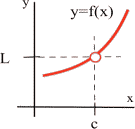
\includegraphics[width=0.24\textwidth]{img/chap2/image011.png} 
\caption{The limit of $f(x)$ as $x\to c$ is $L$.}
\label{fig:2-4-limits}
\vspace{-20pt}
\end{wrapfigure}
The limit of a function describes the behavior (i.e., output) of the function when the variable is near, but not necessarily equal to, a specified number. (See Figure \ref{fig:2-4-limits}.)

\begin{definition}[Limit]
If the values of $f(x)$ get closer and closer, as close as we want, to one single number $L$, as we take values of $x$ very close to (but not equal to) a number $c$, then we say, ``the {\bf limit} of $f(x)$ as $x$ approaches $c$ is $L$'' and we write
$$\lim_{x\to c}f(x)=L \enspace .$$
The symbol ``$\to$'' means ``approaches'' or, less formally, ``gets very close to.''
\end{definition}
This definition of the limit isn't stated as formally as it could be, but it is sufficient for our purposes in this textbook.

{\bf Note:}
    \begin{itemize}[label={}]
    \item $f(c)$ is a single number that describes the behavior (value) of $f(x)$ at the point $x=c$.
    \item $\displaystyle\lim_{x\to c}f(x)$ is a single number that describes the behavior of $f(x)$ near, but NOT at, the point $x=c$.
    \item If we have a graph of $f(x)$ near $x = c$, then it is usually easy to determine $\displaystyle\lim_{x\to c}f(x)$.
    \end{itemize}

\begin{example}
Use the graph of $y=f(x)$ in Figure \ref{fig:2-4-limit-ex} to determine the following limits.
\begin{figure}[!ht]
    \centering
    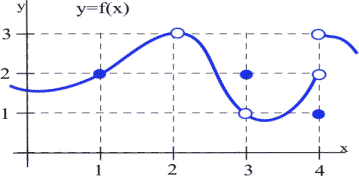
\includegraphics[width=0.4\textwidth]{img/chap2/image012.png}
    \label{$y=f(x)$}
    \label{fig:2-4-limit-ex}
\end{figure}

\begin{enumerate}[label=(\alph*)]
  \item $\displaystyle\lim_{x\to 1}f(x)$

  \begin{solution}
When $x$ is very close to 1, the values of $f(x)$ are very close to $y=2$. In this example, it happens that $f(1)=2$, but that is irrelevant for the limit. The only thing that matters is what happens for $x$ close to 1 but $x\neq 1$.
    \end{solution}
  \item $\displaystyle\lim_{x\to 2}f(x)$

  \begin{solution}
$f(2)$ is undefined, but we only care about the behavior of $f(x)$ for $x$ close to 2 but not equal to 2. When $x$ is close to 2, the values of $f(x)$ are close to 3. If we restrict $x$ close enough to 2, the values of $y$ will be as close to 3 as we want, so $\displaystyle\lim_{x\to 2}f(x)=3$.
    \end{solution}
  \item $\displaystyle\lim_{x\to 3}f(x)$

  \begin{solution}
When $x$ is close to 3 (or ``as $x$ approaches the value 3''), the values of $f(x)$ are close to 1 (or ``approach the value 1''), so $\displaystyle\lim_{x\to 3}f(x)=1$. For this limit it is completely irrelevant that $f(3)=2$. We only care about what happens to $f(x)$ for $x$ close to and not equal to 3.
    \end{solution}
  \item $\displaystyle\lim_{x\to 4}f(x)$

  \begin{solution}
This one is harder and we need to be careful. When $x$ is close to 4 and slightly less than 4 ($x$ is just to the left of 4 on the $x$-axis), then the values of $f(x)$ are close to 2. But if $x$ is close to 4 and slightly larger than 4 then the values of $f(x)$ are close to 3. If we only know that $x$ is very close to 4, then we cannot say whether $y=f(x)$ will be close to 2 or close to 3. It depends on whether $x$ is on the right or the left side of 4. In this situation, the $f(x)$ values are not close to a single number so we say $f(x)$ does not exist. It is irrelevant that $f(4)=1$. The limit, as $x$ approaches 4, would still be undefined if $f(4)$ was 3, 2, or anything else.
    \end{solution}
\end{enumerate}
\end{example}

We can also explore limits using tables and using algebra.

\begin{example}
Find $\displaystyle\lim_{x\to 1}f(x)$, where $f(x) = \dfrac{2x^2-x-1}{x-1}$.

\begin{solution} You might try to evaluate at $x=1$, but $f(x)$ is not defined at $x=1$. It is tempting, but incorrect, to conclude that this function does not have a limit as $x$ approaches 1.

{\bf Using tables:} Trying some ``test'' values for $x$ which get closer and closer to 1 from both the left and the right, we get the following table. 
\begin{table}[ht!]
\begin{centering}
\begin{tabular}{ll||ll}
\toprule
$x$ & 	$f(x)$ & $x$ &	$f(x)$\\					
\midrule
0.9	        & 2.82      & 1.1       & 3.2 \\
0.9998      & 2.9996	& 1.003	    & 3.006 \\
0.999994    & 2.999988	& 1.0001	& 3.0002 \\
0.9999999   & 2.9999998	& 1.000007	& 3.000014 \\
$\to 1$     & $\to 3$   & $\to 1$   & $\to 3$ \\
\bottomrule
\end{tabular}
\caption{Finding the limit of $f(x)$ as $x\to 1$}
\label{tab:2-4-limitex}
\end{centering}
\end{table}
Table \ref{tab:2-4-limitex} suggests that $\displaystyle\lim_{x\to 1}f(x) = 3$. This is not a proof, but is very convincing. A proof would require algebraic techniques.

{\bf Using algebra:} We can prove this result by noting that
$$f(x)=\dfrac{2x^2-x-1}{x-1}=\frac{(2x+1)(x-1)}{x-1}=2x+1 \enspace ,$$
as long as $x\neq 1$. (If $x\neq 1$, then $x-1\neq 0$, so it is valid to divide the numerator and denominator by the factor $x-1$.) The ``$x\to 1$'' part of the limit means that $x$ is close to 1 but not equal to 1, so our division step is valid and
$$\lim_{x\to 1}\dfrac{2x^2-x-1}{x-1}=\lim_{x\to 1}2x+1=3 \enspace,$$
which is our answer.

{\bf Using a graph:} We can graph $y=f(x)=\dfrac{2x^2-x-1}{x-1}$ for $x$ close to 1.
\begin{figure}[!ht]
    \centering
    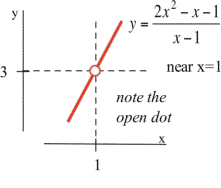
\includegraphics[width=0.4\textwidth]{img/chap2/image013.png}
    \label{$y=f(x)$ near $x=1$}
    \label{fig:2-4-limit-zoom}
\end{figure}
Notice that whenever $x$ is close to 1, the values of $y=f(x)$ are close to 3. Since $f$ is not defined at $x=1$, the graph has a hole above $x=1$, but we only care about what $f(x)$ is doing for $x$ close to but not equal to 1. Therefore,
$$\lim_{x\to 1}\dfrac{2x^2-x-1}{x-1}=\lim_{x\to 1}2x+1=3 \enspace.$$
\end{solution}\end{example}

\subsection{One Sided Limits}
Sometimes, what happens to us at a place depends on the direction we use to approach that place. If we approach Niagara Falls from the upstream side, then we will be 182 feet higher and have different worries than if we approach from the downstream side. Similarly, the values of a function near a point may depend on the direction we use to approach that point.

\definition[Left and Right Limits]
The {\bf left limit}\index{Limit!left} of $f(x)$ as $x$ approaches $c$ is $L$ if the values of $f(x)$ get as close to $L$ as we want when $x$ is very close to and left of $c$ (i.e., $x<c$). We write:
$$\lim_{x\to c^-}f(x)=L \enspace .$$
The{\bf right limit}\index{Limit!right} of $f(x)$ as $x$ approaches $c$ is $L$ if the values of $f(x)$ get as close to $L$ as we want when $x$ is very close to and right of $c$ (i.e., $x>c$). We write
$$\lim_{x\to c^+}f(x)=L \enspace .$$
\begin{example}
Evaluate the one sided limits of the function $f(x)$ graphed below at $x=0$ and $x=1$.

[graph]

\begin{solution} As $x$ approaches 0 from the left, the value of the function is getting closer to 1, so $\displaystyle\lim_{x\to 0^-}f(x)=1$.
As $x$ approaches 0 from the right, the value of the function is getting closer to 2, so $\displaystyle\lim_{x\to 0^+}f(x)=2$.
Notice that since the limit from the left and limit from the right are different, the general limit, $\displaystyle\lim_{x\to 0}f(x)$, does not exist.

At $x$ approaches 1 from either direction, the value of the function is approaching 1, so
$$\lim_{x\to 1^-}f(x)=\lim_{x\to 1^+}f(x)=\lim_{x\to 1}f(x)=1 \enspace.$$
\end{solution}\end{example}

\subsection{Continuity}
\label{ssec:continuity}
A function that is ``friendly'' and doesn't have any breaks or jumps in it is called {\bf continuous}\index{Continuous}. More formally,

\begin{definition}[Continuity at a Point]
A function $f(x)$ is {\bf continuous} at $x=a$ if and only if:
    \begin{enumerate}
    \item $f(a)$ exists,
    \item $\displaystyle\lim_{x\to a}f(x)$ exists, and 
    \item $\displaystyle\lim_{x\to a}f(x)=f(a)$.
    \end{enumerate}
\end{definition}
The graph below illustrates some of the different ways a function can behave at and near a point, and the table contains some numerical information about the function and its behavior.

graph 
\begin{table}[ht!]
\begin{centering}
\begin{tabular}{ccc}
\toprule
$a$	& $f(a)$ &	$\displaystyle\lim_{x\to a}f(x)$ \\		
\midrule
1 &	2 & 2	\\
2 & 1 &	2\\
3 & 2 &	Does not exist (DNE)	\\
4 & Undefined &	2\\
\bottomrule
\end{tabular}
%\caption{}
%\label{tab:2-4-limitex2}
\end{centering}
\end{table}
	
Based on the information in the table, we can conclude that $f(x)$ is continuous at 1 since $\displaystyle\lim_{x\to 1}f(x)=2=f(1)$. We can also conclude from the information in the table that $f(x)$ is not continuous at 2, 3, or 4, because $\displaystyle\lim_{x\to 2}f(x)\neq f(2)$, $\displaystyle\lim_{x\to 3} f(x)\neq f(3)$, and $\displaystyle\lim_{x\to 4} f(x)\neq f(4)$.

The behaviors at $x=2$ and $x=4$ exhibit a hole in the graph, sometimes called a {\bf removable discontinuity}\index{Discontinuity!removeable}, since the graph could be made continuous by changing the value of a single point. The behavior at $x=3$ is called a {\bf jump discontinuity}\index{Discontinuity!jump} or {\bf step discontinuity}\index{Discontinuity!step}, since the graph jumps between two values. Jump discontinuities and vertial asymptotes are both {\bf nonremovable discontinuities}\index{Discontinuity!nonremoveable} because they cannot be fixed by changing the value of a single point.

So which functions are continuous? It turns out pretty much every function you've studied is continuous where it is defined: polynomial, radical, rational, exponential, and logarithmic functions are all continuous where they are defined. Moreover, any sum, difference, or product of continuous functions is also continuous.

This is helpful, because the definition of continuity says that for a continuous function, $\displaystyle\lim_{x\to a}f(x)=f(a)$. That means for a continuous function, we can find the limit by direct substitution (evaluating the function) if the function is continuous at $a$.

\begin{example}
Evaluate using continuity, if possible:
    \begin{enumerate}[label=(\alph*)]
    \item $\displaystyle\lim_{x\to 2}x^3-4x$

    \begin{solution} The given function is a polynomial, so it is defined for all values of $x$. Therefore, we can find the limit by direct substitution:
    $$\lim_{x\to 2}x^3-4x = 2^3-4(2) = 0 \enspace.$$
    \end{solution}
    \item $\displaystyle\lim_{x\to 2}\frac{x-4}{x+3}$

    \begin{solution} 
    The given function is rational. It is not defined at $x = -3$, but we are taking the limit as $x$ approaches 2, and the function is defined at that point, so we can use direct substitution:
    $$\lim_{x\to 2}\frac{x-4}{x+3} = \frac{2-4}{2+3}=-\frac{2}{5} \enspace .$$
    \end{solution}
    \item $\displaystyle\lim_{x\to 2} \frac{x-4}{x-2}$

    \begin{solution} 
    This function is not defined at $x = 2$, so is not continuous at $x = 2$. We cannot use direct substitution. There is also no factor of $x-2$ in the numerator, so the $x-2$ in the denominator cannot be canceled out to remove the discontinuity. Therefore, the limit does not exist.
    \end{solution}
\end{enumerate}
\end{example}

\section{Finding Derivatives Algebraically}
\label{sec:algderiv}

Formal Algebraic Definition
f′(x)=limh→0f(x+h)-f(x)h
Practical Definition
The derivative can be approximated by looking at an average rate of change, or the slope of a secant line, over a very tiny interval. The tinier the interval, the closer this is to the true instantaneous rate of change, slope of the tangent line, or slope of the curve.

\begin{example}
Find the slope of the tangent line to f(x)=1x at x=3.

\begin{solution} The slope of the tangent line is the value of the derivative f′(3). f(3)=13 and f(3+h)=13+h, so, using the formal limit definition of the derivative,
f′(3)=limh→0f(3+h)-f(3)h=limh→013+h-13h.
We can simplify by giving the fractions a common denominator:
limh→013+h-13h=======limh→013+h⋅33-13⋅3+h3+hhlimh→039+3h-3+h9+3hhlimh→03-(3+h)9+3hhlimh→03-3-h9+3hhlimh→0-h9+3hhlimh→0-h9+3h⋅1hlimh→0-19+3h
and the evaluate using direct substitution:
limh→0-19+3h=-19+3(0)=-19.
Thus, the slope of the tangent line to f(x)=1x at x=3 is -19.
\end{solution}\end{example}

\begin{example}
Find ddx(2x2-4x-1).

\begin{solution} Setting up the derivative using a limit,
f′(x)=limh→0f(x+h)-f(x)h.
We will start by simplifying f(x+h) by expanding:
f(x+h)===2(x+h)2-4(x+h)-12(x2+2xh+h2)-4(x+h)-12x2+4xh+2h2-4x-4h-1
Now finding the limit:
f′(x)======limh→0f(x+h)-f(x)hlimh→0(2x2+4xh+2h2-4x-4h-1)-(2x2-4x-1)hlimh→02x2+4xh+2h2-4x-4h-1-2x2+4x+1h(Substitute in the formulas.)limh→04xh+2h2-4hh(Now simplify.)limh→0h(4x+2h-4)h(Factor out the h, then cancel.)limh→0(4x+2h-4)
We can find the limit of this expression by direct substitution:
f′(x)=limh→0(4x+2h-4)=4x-4
Notice that the derivative depends on x, and that this formula will tell us the slope of the tangent line to f at any value x. For example, if we wanted to know the tangent slope of f at x=3, we would simply evaluate: f′(3)=4(3)-4=8.
\end{solution}\end{example}
A formula for the derivative function is very powerful, but as you can see, calculating the derivative using the limit definition is very time consuming. In the next section, we will identify some patterns that will allow us to start building a set of rules for finding derivatives without needing the limit definition.

\section{Sum, Difference, and Constant Multiple Rules}
\label{sec:power}

In the next few sections, we'll get the derivative rules that will let us find formulas for derivatives when our function comes to us as a formula. 

\subsection{Sum and Difference}
Given two functions, $f(x)$ and $g(x)$, what can be said about the derivative of their sum? Think about it. What should we expect for the slope of the curve $y = f(x)+g(x)$ or the curve $y=f(x) - g(x)$? We can prove the following result using the limit definition of the derivative, but it should make intuitive sense that the slope of a sum is the sum of the slopes.

\begin{theorem}[Sum and Difference Rule\index{Sum and difference rule}\index{Derivative rules!Sum and difference rule}]
\label{thm:sumdiffderiv}
If $f(x)$ and $g(x)$ are differentiable, then 
    $$\dfrac{d}{dx}(f(x) \pm g(x))=f'(x) \pm g'(x) \enspace .$$
\end{theorem}

\subsection{Constant Multiples}
Given a single function, $f(x)$, we have $2f(x) = f(x) + f(x)$ and $3f(x) = f(x) + f(x) + f(x)$, so it would make sense that the slope of $y=k\cdot f(x)$ is $k$ times the slope of $y=f(x)$. This too, can be proved using the limit definition of the derivative. We often say that when taking the derivative of a multiple of a function, that ``constants come along for the ride.'' 

\begin{theorem}[Constant Multiple Rule\index{Constant multiple rule}\index{Derivative rules!Constant multiple rule}]
\label{thm:constmultderiv}
If $f(x)$ is differentiable and $k$ is a real number, then
$$\dfrac{d}{dx}(k\cdot f(x))=k\cdot f'(x) \enspace .$$
\end{theorem}

\subsection{Exercises}
\begin{enumerate}
    \item Prove Theorem \ref{thm:sumdiffderiv} using the limit definition of the derivative, Definition \ref{def:deriv}.
    \item Prove Theorem \ref{thm:constmultderiv} using the limit definition of the derivative, Definition \ref{def:deriv}.
\end{enumerate}


\section{The Power Rule}
\label{sec:power}

\section{Exponential and Logarithmic Functions}
\label{sec:explogderiv}

\begin{theorem}
{\bf Exponential Functions}
$$\dfrac{d}{dx}e^x=e^x$$
$$\dfrac{d}{dx}a^x=\ln(a)a^x$$
{\bf Logarithmic Functions}
$$\dfrac{d}{dx}\ln(x)=\dfrac{1}{x}$$
$$\dfrac{d}{dx}\log_b(x)=\dfrac{1}{x\ln(b)}\enspace , b>0, b\neq 1 $$
\end{theorem}

\section{The Product and Quotient Rules}
\label{sec:prod-quot}

% Dollar-cost averaging example. Invest $100 per month and price of asset goes up \$10 per month. How fast does the investment grow?

The basic rules will let us tackle simple functions. But what happens if we need the derivative of a combination of these functions?

\begin{example}
  \label{ex:2-8-1}
Find the derivative of $h(x)=(4x^3-11)(x+3)$.

\begin{solution} This function is not a simple sum or difference of polynomials. It's a product of polynomials. We can simply multiply it out to find its derivative:
\begin{align*}
		h(x) &= \left(4x^3-11\right)(x+3)\\
		 &= 4x^4-11x+12x^3-33\\
		h'(x) &= 16x^3-11+36x^2
	\end{align*}
\end{solution}\end{example}

Now suppose we wanted to find the derivative of
$$f(x)=\left(4x^5+x^3-1.5x^2-11\right)\left(x^7-7.25x^5+120x+3\right)$$)
This function is not a simple sum or difference of polynomials. It's a product of polynomials. We could 'simply' multiply it out to find its derivative as before -- who wants to volunteer? Nobody?

We'll need a rule for finding the derivative of a product so we don't have to multiply everything out.

It would be great if we can just take the derivatives of the factors and multiply them, but unfortunately that won't give the right answer. To see that, consider finding derivative of $h(x)=(4x^3-11)(x+3)$. We already worked out the derivative, it is $h'(x)=16x^3-11+36x^2$. What if we try differentiating the factors and multiplying them? We'd get $h'(x)=(12x^2)(1)=12x^2$, which is radically different from the correct answer.

In other words, the derivative of a product is not the product of the derivatives.

The rules for finding derivatives of products and quotients are a little complicated, but they save us the much more complicated algebra we might face if we were to try to multiply things out. They also let us deal with products where the factors are not polynomials. We can use these rules, together with the basic rules, to find derivatives of many complicated looking functions.

\subsection{Derivative Rules: Product and Quotient Rules}
\begin{theorem}[Product Rule\index{Product Rule}]
If $f(x)$ and $g(x)$ are differentiable, then
$\dfrac{d}{dx}\left( f(x)\cdot g(x) \right)=f'(x)\cdot g(x)+f(x)\cdot g'(x) \enspace .$
\end{theorem}

The derivative of the first factor times the second left alone, plus the first left alone times the derivative of the second.

The Product Rule can extend to a product of several functions; the pattern continues -- take the derivative of each factor in turn, multiplied by all the other factors left alone, and add them up:
$$\dfrac{d}{dx} f(x)\cdot g(x)\cdot h(x) = f'(x)\cdot g(x)\cdot h(x)+f(x)\cdot g'(x)\cdot h(x)+f(x)\cdot g(x)\cdot h'(x)$$


\begin{theorem}[Quotient Rule\index{Quotient Rule}]
$$\dfrac{d}{dx}\dfrac{f(x)}{g(x)} = \dfrac{f'(x)\cdot g(x)-f(x)\cdot g'(x)}{g^2(x)}$$
\end{theorem}
An easy way to remember this is with a chant.\\

``Low dee high

minus high dee low

over low squared

it's the way to go.''

The numerator of the result resembles the Product Rule, but there is a minus instead of a plus; the minus sign goes with the $g'(x)$. The denominator is simply the square of the original denominator -- no derivatives there.

\begin{example}
Find the derivative of $h(x)=(4x^3-11)(x+3)$

\begin{solution} This is the same function we found the derivative of in Example \ref{ex:2-8-1} , but let's use the Product Rule and check to see if we get the same answer. For this first example, we will provide a lot more detail and steps than one usually actually shows when working a problem like this.

Notice we can think of $h(x)$ as the product of two functions $f(x)=4x^3-11$ and $g(x)=x+3$. Finding the derivative of each of these,
$f'(x)=12x^2$ and $g'(x)=1$.
Using the Product Rule, we have: 
\begin{align*}
		h'(x) &= (f')(g)+(f)(g') \\
		 &= \left(12x^2\right)(x+3)+\left(4x^3-11\right)(1)
	\end{align*}
To check if this is equivalent to the answer we found in Example \ref{ex:2-8-1}  we could simplify:
\begin{align*}
		h'(x) &= \left(12x^2\right)(x+3)+\left(4x^3-11\right)(1) \\
		 &= 12x^3+36x^2+4x^3-11 \\
		 &= 16x^3+36x^2-11
	\end{align*}
From this, we can see the answers are equivalent.
\end{solution}\end{example}

\begin{example}
Find the derivative of $ F(t)=e^t\ln(t) $.

\begin{solution} This is a product, so we need to use the Product Rule. 
$$F'(t)=\left(e^t\right)\left(\ln(t)\right)+\left(e^t\right)\left(\dfrac{1}{t}\right)=e^t\ln(t)+\dfrac{e^t}{t}$$
\end{solution}\end{example}

Notice that this was one we could not have done by multiplying out.

\begin{example}
Find the derivative of $ y=\dfrac{x^4+4^x}{3+16x^3} $.

\begin{solution} This is a quotient, so we need to use the Quotient Rule.
$$y'=\dfrac{\left(4x^3+\ln(4)\cdot 4^x \right)\left(3+16x^3 \right)-\left(x^4+4^x \right)\left(48x^2 \right)}{\left(3+16x^3 \right)^2}$$
\end{solution}\end{example}

Now for goodness' sake don't try to simplify that! Remember that simple depends on what you will do next; in this case, we were asked to find the derivative, and we've done that. I expect you to do any basic simplifications, such as multiplying constants together or doing obvious cancellations or combining of terms, but otherwise please STOP unless there is a reason to simplify further.

\begin{example}
Suppose a large tank contains 8 kg of a chemical dissolved in 50 liters of water. If a tap is opened and water is added to the tank at a rate of 5 liters per minute, at what rate is the concentration of chemical in the tank changing after 4 minutes?

\begin{solution} First we need to set up a model for the concentration of chemical. The concentration would be measured as kg of chemical per liter of water, kg/L. The number of kg of chemical stays constant at 8 kg, but the quantity of water in the tank is increasing at a constant rate of 5 L/min. The total volume of water in the tank after t minutes is $50+5t$, so the concentration after $t$ minutes is
$$c(t)=\dfrac{8}{50+5t} \enspace .$$
To find the rate at which the concentration is changing, we need the derivative:
\begin{align*}
			c'(t) &= \dfrac{\dfrac{d}{dt}(8)\cdot(50+5t)-(8)\cdot\dfrac{d}{dt}(50+5t)}{(50+5t)^2} \\
			 &= \dfrac{(0)\cdot(50+5t)-(8)(5)}{(50+5t)^2} \\
			 &= -\dfrac{40}{(50+5t)^2} \enspace .
		\end{align*}
At $t=4$ minutes, we have 
$$ c'(4)=-\dfrac{40}{(50+5(4))^2}\approx -0.00816 \enspace .$$
Note that the units here are kg per liter, per minute, or $ \dfrac{\text{kg/L}}{\text{min}} $. In other words, this tells us that after 4 minutes, the concentration of chemical is decreasing at a rate of 0.00816 kg/L per minute.
\end{solution}\end{example}

\subsection{More Graphical Interpretations of the Basic Business Math Terms}
Returning to our discussion of business and economics topics, in addition to total cost\index{Cost} and marginal cost\index{Marginal cost}, we often also want to talk about average cost\index{Average cost}\index{Cost!average} or average revenue\index{Average revenue}\index{Revenue!average}.

Recall from Section \ref{sec:functions} (Definition \ref{def:avgcost} that the average cost for $q$ items is the total cost divided by $q$, or $A(q)=\dfrac{C(q)}{q}$. You can also talk about the average fixed cost, $\dfrac{FC(q)}{q}$, or the average variable cost, $\dfrac{VC(q)}{q}$.

Also recall that the Average Revenue (AR) for $q$ items is the total revenue divided by $q$, or $AR(q)=\dfrac{R(q)}{q}$. But $\dfrac{R(q)}{q} = \dfrac{q \cdot D(q)}{q}= D(q)$, so $AR(q)=D(q)$, which just the price since $p=D(q)$.

We already know that we can find average rates of change by finding slopes of secant lines. AC, AR, MC, and MR are all rates of change, and we can find them with slopes too.

$AC(q)$ is the slope of a diagonal line, from $(0, 0)$ to $(q,C(q))$.

$AR(q)$ is the slope of the line from $(0, 0)$ to $(q,R(q))$, which is the also equal to the price at $(q,R(q))$ by the calulations in the previous paragraph.

\begin{figure}[!ht]
  \centering
    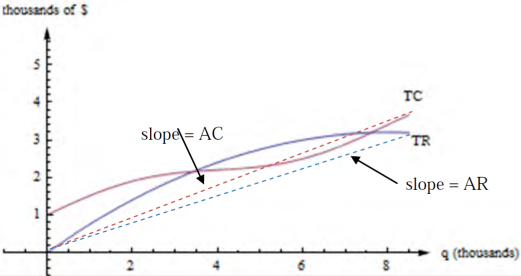
\includegraphics[width=0.4\textwidth]{img/chap2/image113.png}
    %\caption{$y=g(x)$}
    %\label{fig:2-2-gx}
\end{figure}

And just as we found marginal Total Cost, we can also find marginal Average Cost.

\begin{example}
The cost, in thousands of dollars, for producing $x$ thousand cellphone cases is given by $C(x)=22+x-0.004x^2$. Find
    \begin{enumerate}[label=(\alph*)]
    \item the Fixed Costs,
    \begin{solution}
    The fixed costs are the costs when no items are produced: $C(0)=22$ thousand dollars.
    \end{solution}
    \item the Average Cost when 5 thousand, 10 thousand, or 20 thousand cases are produced,
    \begin{solution}
    The average cost function is total cost divided by number of items, so
$$AC(x)=\dfrac{C(x)}{x}=\dfrac{22+x-0.004x^2}{x}. $$
Note the units are thousands of dollars per thousands of items, which simplifies to just dollars per item.

At a production of 5 thousand items: $ AC(5)=\dfrac{22+5-0.004(5)^2}{5}=5.38 $ dollars per item.

At a production of 10 thousand items: $ AC(10)=\dfrac{22+5-0.004(10)^2}{10}=3.16 $ dollars per item.

At a production of 20 thousand items: $ AC(20)=\dfrac{22+5-0.004(20)^2}{20}=2.02 $ dollars per item.

Notice that while the total cost increases with production, the average cost per item decreases, because the initial fixed costs are being distributed across more items.
    \end{solution}
    \item the Marginal Average Cost when 5 thousand cases are produced.

    \begin{solution} 
    For the marginal average cost, we need to find the derivative of the average cost function. We can either calculate this using the Quotient Rule, or we could use algebra to simplify the equation first (this is the easier option -- remember, simplifying before differentiating is almost always easier):
    \begin{align*}
					AC(x) &= \dfrac{22+x-0.004x^2}{x} \\
					 &= \dfrac{22}{x}+\dfrac{x}{x}-\dfrac{0.004x^2}{x} \\
					 &= \dfrac{22}{x}+1-0.004x \\
					 &= 22
\end{align*}
(Note: we haven't differentiated yet, only simplified.)

Taking the derivative,
$$ AC'(x)=-22x^{-2}-0.004=-\dfrac{22}{x^2}-0.004 \enspace .$$
When 5 thousand items are produced,
$$ AC'(5)=-\dfrac{22}{5^2}-0.004=-0.884 \enspace .$$
Since the units on $AC(x)$ are dollars per item, and the units on $x$ are thousands of items, the units on $AC'(x)$ are dollars per item per thousands of items. This tells us that when 5 thousand items are produced, the average cost per item is decreasing at a rate of \$0.884 per additional thousand items produced.
    \end{solution}
    \end{enumerate}
\end{example}

%\section{The Chain Rule}
\label{sec:chain}

There is one more type of complicated function that we will want to know how to differentiate: composition. The Chain Rule will let us find the derivative of a composition. (This is the last derivative rule we will learn!)

\begin{example}
Find the derivative of y=(4x3+15x)2
\begin{solution} This is not a simple polynomial, so we can’t use the basic building block rules yet. It is a product, so we could write it as y=(4x3+15x)2=(4x3+15x)(4x3+15x) and use the product rule. Or we could multiply it out and simply differentiate the resulting polynomial. I’ll do it the second way:
y==y′=(4x3+15x)216x6+120x4+225x296x5+480x3+450x
\end{solution}\end{example}

Now suppose we want to find the derivative of y=(4x3+15x)20. We could write it as a product with 20 factors and use the product rule, or we could multiply it out. But I don't want to do that, do you?

We need an easier way, a rule that will handle a composition like this. The Chain Rule is a little complicated, but it saves us the much more complicated algebra of multiplying something like this out. It will also handle compositions where it wouldn't be possible to multiply it out.

The Chain Rule is a common place for students to make mistakes. Part of the reason is that the notation takes a little getting used to. And part of the reason is that students often forget to use it when they should. When should you use the Chain Rule? Almost every time you take a derivative.

Derivative Rules: Chain Rule
In what follows, f and g are differentiable functions with y=f(u) and u=g(x).

Chain Rule (Leibniz notation)
dydx=dydu⋅dudx
Notice that the du’s seem to cancel. This is one advantage of the Leibniz notation – it can remind you of how the chain rule chains together.

Chain Rule (using prime notation)
ddx[f(g(x))]=f′(u)⋅g′(x)=f′(g(x))⋅g′(x)
Chain Rule (in words)
The derivative of a composition is the derivative of the outside (with the inside staying the same) TIMES the derivative of the inside.

I recite the version in words each time I take a derivative, especially if the function is complicated.

\begin{example}
Find the derivative of y=(4x3+15x)2
\begin{solution} This is the same one we did before by multiplying out. This time, let’s use the Chain Rule: The inside function is what appears inside the parentheses: 4x3+15x. The outside function is the first thing we find as we come in from the outside – it’s the square function, (inside)2.

The derivative of this outside function is (2⋅inside). Now using the chain rule, the derivative of our original function is (2⋅inside) TIMES the derivative of the inside (which is 12x2+15):
y′=2(4x3+15x)(12x2+15)
\end{solution}\end{example}

If you multiply this out, you get the same answer we got before. Hurray! Algebra works!

\begin{example}
Find the derivative of y=(4x3+15x)20.

\begin{solution} Now we have a way to handle this one. It’s the derivative of the outside TIMES the derivative of the inside.

The outside function is (inside)20, which has derivative 20(inside)19, so
y′=20(4x3+15x)19(12x2+15).
\end{solution}\end{example}

\begin{example}
Differentiate y=ex2+5.

\begin{solution} This isn’t a simple exponential function; it’s a composition. Typical calculator or computer syntax can help you see what the “inside” function is here. On a TI calculator, for example, when you push the ex key, it opens up parentheses: e^( . This tells you that the "inside" of the exponential function is the exponent. Here, the inside is the exponent x2+5. Now we can use the Chain Rule: We want the derivative of the outside TIMES the derivative of the inside. The outside is the e to the something function, so its derivative is the same thing. The derivative of what’s inside is 2x. So
ddx(ex2+5)=(ex2+5)⋅(2x).
\end{solution}\end{example}

\begin{example}
The table gives values for f , f′ , g, and g′ at a number of points. Use these values to determine (f∘g)(x) and (f∘g)′(x) at x=-1 and 0.

x	f(x)	g(x)	f′(x)	g′(x)	(f∘g)(x)	(g∘f)(x)	-1	2	3	1	0			0	-1	1	3	2			1	1	0	-1	3			2	3	-1	0	1			3	0	2	2	-1
\begin{solution} (f∘g)(-1)=(f∘g)(0)=(f∘g)′(-1)=(f∘g)′(0)=f(g(-1))=f(3)=0f(g(0))=f(1)=1f′(g(-1))⋅g′(-1)=f′(3)⋅(0)=(2)(0)=0 andf′(g(0))⋅g′(0)=f′(1)⋅(2)=(-1)(2)=-2
\end{solution}\end{example}

\begin{example}
If 2400 people now have a disease, and the number of people with the disease appears to double every 3 years, then the number of people expected to have the disease in t years is y=2400⋅2t/3.

How many people are expected to have the disease in 2 years?
When are 50,000 people expected to have the disease?
How fast is the number of people with the disease expected to grow now and 2 years from now?
\begin{solution} In 2 years, y=2400⋅22/3\approx   3,810 people.
We know y=50,000, and we need to solve 50,000=2400⋅2t/3 for t. We could start by isolating the exponential by dividing both sides by 2400,
500002400=ln(500002400)=ln(500002400)=t=2t/3ln(2t/3)(Taking the natural log of both sides.)t3ln(2)(Using the exponent property for logs.)3ln(500002400)ln(2)\approx   13.14 years(Solving for t.)
We expect 50,000 people to have the disease about 13.14 years from now.
This is asking for dydt when t= 0 and 2 years. Using the chain rule,
dydt==\approx   ddt(2400⋅2t/3)2400⋅2t/3⋅ln(2)⋅13554.5⋅2t/3
So, at t=0 the rate of growth of the disease is approximately 554.5⋅20\approx   554.5 people/year. In 2 years the rate of growth will be approximately 554.5⋅22/3\approx   880 people/year.
\end{solution}\end{example}

Derivatives of Complicated Functions
You're now ready to take the derivative of some mighty complicated functions. But how do you tell what rule applies first? Work your way in from the outside – what do you encounter first? That’s the first rule you need. Use the Product, Quotient, and Chain Rules to peel off the layers, one at a time, until you’re all the way inside.

\begin{example}
Find ddx(e3x⋅ln(5x+7))
\begin{solution} Coming in from the outside, we see that this is a product of two (complicated) functions. So we’ll need the Product Rule first. we’ll fill in the pieces we know, and then we can figure the rest as separate steps and substitute in at the end:
ddx(e3x⋅ln(5x+7))=(ddx(e3x))⋅ln(5x+7)+e3x⋅(ddx(ln(5x+7)))
Now as separate steps, we’ll find
ddx(e3x)=3e3x (using the Chain Rule)
and
ddx(ln(5x+7))=15x+7⋅5 (also using the Chain Rule).
Finally, to substitute these in their places:
ddx(e3x⋅ln(5x+7))=(3e3x)⋅ln(5x+7)+e3x⋅(15x+7⋅5)
(We can stop here – we don't need to try to simplify any further.)
\end{solution}\end{example}

\begin{example}
Differentiate z=(3t3et(t-1))4
\begin{solution} Don’t panic! As we come in from the outside, what’s the first thing we encounter? It’s that fourth power. That tells us that this is a composition, a (complicated) function raised to the fourth power.

Step One: Use the Chain Rule. The derivative of the outside TIMES the derivative of the inside:
dzdt=ddt(3t3et(t-1))4=4(3t3et(t-1))3⋅ddt(3t3et(t-1))
Now we’re one step inside, and we can concentrate on just the ddt(3t3et(t-1)) part. Now, as you come in from the outside, the first thing you encounter is a quotient – this is the quotient of two (complicated) functions.

Step Two: Use the Quotient Rule. The derivative of the numerator is straightforward, so we can just calculate it. The derivative of the denominator is a bit trickier, so we'll leave it for now:
ddt(3t3et(t-1))=(9t2)(et(t-1))-(3t3)(ddt(et(t-1)))(et(t-1))2
Now we’ve gone one more step inside, and we can concentrate on just the ddt(et(t-1)) part, which involves a product.

Step Three: Use the Product Rule:
ddt(et(t-1))=(et)(t-1)+(et)(1)
And now we’re all the way in – no more derivatives to take!

Step Four: Now it’s just a question of substituting back – be careful now!

ddt(et(t-1))=(et)(t-1)+(et)(1)
so
ddt(3t3et(t-1))=(9t2)(et(t-1))-(3t3)((et)(t-1)+(et)(1))(et(t-1))2
so
dzdt=ddt(3t3et(t-1))4=4(3t3et(t-1))3⋅((9t2)(et(t-1))-(3t3)((et)(t-1)+(et)(1))(et(t-1))2)
Phew!
\end{solution}\end{example}

What if the Derivative Doesn’t Exist?
Differentiable
A function is called differentiable at a point if its derivative exists at that point.

We’ve been acting as if derivatives exist everywhere for every function. This is true for most of the functions that you will run into in this class. But there are some common places where the derivative doesn’t exist.

Remember that the derivative is the slope of the tangent line to the curve. That’s what to think about.

Where can a slope not exist? If the tangent line is vertical, the derivative will not exist.

\begin{example}
Show that f(x)=x--√3=x1/3 is not differentiable at x=0.

\begin{solution} Finding the derivative, f′(x)=13x-2/3=13x2/3. At x=0, this function is undefined. From the graph, we can see that the tangent line to this curve at x=0 is vertical with undefined slope, which is why the derivative does not exist at x=0.

graph
\end{solution}\end{example}

Where can a tangent line not exist?

If there is a sharp corner (cusp) in the graph, the derivative will not exist at that point because there is no well-defined tangent line (a teetering tangent, if you will).

If there is a discontinuity in the graph (a jump, a break, a hole in the graph, or a vertical asymptote), the tangent line will be different on either side and the derivative will not exist at that point.

\begin{example}
Show that f(x)=|x| is not differentiable at x=0.

\begin{solution} On the left side of the graph, the slope of the line is -1. On the right side of the graph, the slope is +1. There is no well-defined tangent line at the sharp corner at x=0, so the function is not differentiable at that point.

graph
\end{solution}\end{example}

\section{Trigonometric Functions}
\label{sec:trigderiv}

\subsection{Derivative Formulas}

\begin{theorem}
$$\dfrac{d}{dx}\sin(x) = \cos(x)$$

$$\dfrac{d}{dx}\cos(x) = -\sin(x)$$
\end{theorem}

From this, we can figure out the derivatives of the four other trigonometric functions.

\begin{theorem}
$$\dfrac{d}{dx}\tan(x) = \sec^2(x)$$
\end{theorem}
\begin{proof}
Here, we'll use the fact that $\tan(x) = \dfrac{\sin(x)}{\cos(x)}$ and use the Quotient Rule, since we are finding the derivative of a quotient (fraction).
\begin{align*}
    \dfrac{d}{dx}\tan(x) &= \dfrac{d}{dx}\frac{\sin(x)}{\cos(x)} \\
    &= \dfrac{\cos(x)\cdot\frac{d}{dx}\sin(x) - \sin(x)\cdot\frac{d}{dx}\cos(x)}{\cos^2(x)} \\
    &= \dfrac{\cos(x)\cdot\cos(x) - \sin(x)\cdot(-\sin(x))}{\cos^2(x)} \\
    &= \dfrac{\cos^2(x) + \sin^2(x)}{\cos^2(x)} \\
    &= \dfrac{1}{\cos^2(x)}\\
    &= \sec^2(x)
\end{align*}
\end{proof}

\subsection{Examples}

\subsection{Exercises}

%\section{Higher Order Derivatives}
\label{sec:higherorder}

\subsection{Second Derivative}
\label{ssec:second-deriv}

Let y=f(x). The second derivative of f is the derivative of y′=f′(x).

Using prime notation, this is f′′(x) or y′′. You can read this aloud as "f double prime of x" or "y double prime."

Using Leibniz notation, the second derivative is written d2ydx2 or d2fdx2. This is read aloud as "the second derivative of y (or f)."

If f′′(x) is positive on an interval, the graph of y=f(x) is concave up on that interval. We can say that f is increasing (or decreasing) at an increasing rate.

If f′′(x) is negative on an interval, the graph of y=f(x) is concave down on that interval. We can say that f is increasing (or decreasing) at a decreasing rate.

\begin{example}
Find f′′(x) for f(x)=3x7.

\begin{solution} First, we need to find the first derivative:
f′(x)=21x6.
Then we take the derivative of that function:
f′′(x)=ddx(f′(x))=ddx(21x6)=126x5.
\end{solution}\end{example}

If f(x) represents the position of a particle at time x, then v(x)=f′(x) will represent the velocity (rate of change of the position) of the particle and a(x)=v′(x)=f′′(x) will represent the acceleration (the rate of change of the velocity) of the particle.

You are probably familiar with acceleration from driving or riding in a car. The speedometer tells you your velocity (speed). When you leave from a stop and press down on the accelerator, you are accelerating – increasing your speed.

\begin{example}
The height (feet) of a particle at time t seconds is f(t)=t3–4t2+8t. Find the height, velocity and acceleration of the particle when t= 0, 1, and 2 seconds.

\begin{solution} f(t)=t3–4t2+8t so f(0)=0 feet, f(1)=5 feet, and f(2)=8 feet.

The velocity is v(t)=f′(t)=3t2–8t+8 so v(0)=8 ft/s, v(1)=3 ft/s, and v(2)=4 ft/s. At each of these times the velocity is positive and the particle is moving upward, increasing in height.

The acceleration is a(t)=f′′(t)=6t–8 so a(0)=–8 ft/s2, a(1)=–2 ft/s2 and a(2)=4 ft/s2.

At time 0 and 1, the acceleration is negative, so the particle's velocity would be decreasing at those points - the particle was slowing down. At time 2, the velocity is positive, so the particle was increasing in speed.
\end{solution}\end{example}

